\chapter{Nestor2: dumping of supply material}
%
%****************************************************
% - Purpose & Problem description:
%     These first two parts give reader short details about the test case,
%     the physical phenomena involved and specify how the numerical solution will be validated
\section{Purpose (Dump\_by\_time)}
%
Example for Nestor:\\
dumping of supply material\\
\\
Details about:
\begin{itemize}
\item{\texttt{ActionType = Dump\_by\_time}}
\item{Convention for the supply material \texttt{GrainClass~~~}} \,see chpt.\,\ref{ssec:E1SuppMat} (page \pageref{txt:SupplyMaterial})
%\item{\texttt{DumpPlanar~=~TRUE/FALSE~~~}} for more details see page \pageref{txt:DumpPlanar}
%\item{\texttt{ReferenceLevel~=~SECTIONS~}} for more details see page \pageref{txt:Reflevel}
\item{\texttt{DumpPlanar~=~TRUE/FALSE~~~}} for more details see chpt.\,\ref{ssec:DumpPlanar} (page \pageref{txt:DumpPlanar})
\item{\texttt{ReferenceLevel~=~SECTIONS~}} for more details see chpt.\,\ref{ssec:E4RefLev} (page \pageref{txt:Reflevel})
\end{itemize}



\newpage
%****************************************************
\section{Description of the problem}
%
This example performs two actions of dumping supply material.
One is running with the dumping mode \texttt{DumpPlanar~=~FALSE}.
The other is running with \texttt{DumpPlanar~=~TRUE}.
Two dumping areas are defined by polygons which are defined in file \texttt{\_DigPolys.dat}.
Both are located in the larger wide section between meter 615,5 and 766,5 (fig.\,\ref{E2ini}).
The area of each polygon is 1173 m$^2$ and covers a hollow in the bottom.
The deepest points in the hollows are 3\,m below the plane bottom (fig.\,\ref{E2result3D}).\\
\\
\subsection{Action-1: Dump with DumpPlanar = FALSE}
Excerpt from the action file where Action-1 is defined:\\
\hspace*{3mm} \texttt{\small{~~~:}}\\
\hspace*{3mm} \texttt{\small{/================================================================}}\\
\hspace*{3mm} \texttt{\small{ACTION}}                                                           \\
\hspace*{3mm} \texttt{\small{~~~ActionType~~~=~~~~Dump\_by\_time}}                              \\
\hspace*{3mm} \texttt{\small{~~~}}                                                              \\
\hspace*{3mm} \texttt{\small{~~~TimeStart~~~~=~~2000.01.01-00:00:02~~~~/~[yyyy.mm.dd-hh:mm:ss]}}\\
\hspace*{3mm} \texttt{\small{~~~TimeEnd~~~~~~=~~2000.01.01-00:02:02~~~~/~[yyyy.mm.dd-hh:mm:ss]}}\\
\hspace*{3mm} \texttt{\small{~~~}}                                                              \\
\hspace*{3mm} \texttt{\small{~~~FieldDump~~~~=~~~401\_hollow1\_1173m**2}}                       \\
\hspace*{3mm} \texttt{\small{~~~DumpPlanar~~~=~~~FALSE~}}                                       \\
\hspace*{3mm} \texttt{\small{~~~}}                                                              \\
\hspace*{3mm} \texttt{\small{~~~DumpVolume~~~=~~586.50~~~~~~~~~~~~~~~~~/~[~m**3~]}}             \\
\hspace*{3mm} \texttt{\small{~~~GrainClass~~~=~~~~0.2}}                                         \\
\hspace*{3mm} \texttt{\small{~~~GrainClass~~~=~~~~0.1}}                                         \\
\hspace*{3mm} \texttt{\small{~~~GrainClass~~~=~~~~0.0}}                                         \\
\hspace*{3mm} \texttt{\small{~~~GrainClass~~~=~~~~0.7}}                                         \\
\hspace*{3mm} \texttt{\small{ENDACTION}}                                                        \\
\hspace*{3mm} \texttt{\small{/================================================================}}\\
\hspace*{3mm} \texttt{\small{~~~:}}\\
\\
Over a time period of 120\,s 586.5 m$^3$ supply material will be dumped in the polygon named
\texttt{~401\_hollow1\_1173m**2~}. Due to the setting \texttt{~DumpPlanar~=~FALSE~} all the nodes
in the area will elevate about the same value (fig.\,\ref{E4PlanF}); In this case about 0.5 m.
The composition of the supply material is defined through the multiple use of the keyword \texttt{GrainClass}
(convention for supply material: chpt.\,\ref{ssec:E1SuppMat}\,/\,page \pageref{txt:SupplyMaterial}).\\
Here the supply material is composed of the two finest and the most coarse fraction of the bed sediment.
Because the 3rd grain class is not part of the supply material it is set to 0.\\


\newpage

\subsection{Action-2: Dump with DumpPlanar = TRUE}
Excerpt from the action file where Action-2 is defined:\\
\hspace*{3mm} \texttt{\small{~~~:}}\\
\hspace*{3mm} \texttt{\small{/================================================================}}\\
\hspace*{3mm} \texttt{\small{ACTION}}                                                           \\
\hspace*{3mm} \texttt{\small{~~~ActionType~~~~~~=~~~Dump\_by\_time}}                            \\
\hspace*{3mm} \texttt{\small{~~~}}                                                              \\
\hspace*{3mm} \texttt{\small{~~~TimeStart~~~~~~~=~2000.01.01-00:00:02~~/~[yyyy.mm.dd-hh:mm:ss]}}\\
\hspace*{3mm} \texttt{\small{~~~TimeEnd~~~~~~~~~=~2000.01.01-00:02:02~~/~[yyyy.mm.dd-hh:mm:ss]}}\\
\hspace*{3mm} \texttt{\small{~~~}}                                                              \\
\hspace*{3mm} \texttt{\small{~~~FieldDump~~~~~~~=~~402\_hollow1\_1173m**2}}                     \\
\hspace*{3mm} \texttt{\small{~~~DumpPlanar~~~~~~=~~TRUE~}}                                      \\
\hspace*{3mm} \texttt{\small{~~~ReferenceLevel~~=~~SECTIONS}}                                   \\
\hspace*{3mm} \texttt{\small{~~~}}                                                              \\
\hspace*{3mm} \texttt{\small{~~~DumpVolume~~~~~~=~586.50~~~~~~~~~~~~~~~~~/~[~m**3~]}}           \\
\hspace*{3mm} \texttt{\small{~~~GrainClass~~~~~~=~~~0.2}}                                       \\
\hspace*{3mm} \texttt{\small{~~~GrainClass~~~~~~=~~~0.1}}                                       \\
\hspace*{3mm} \texttt{\small{~~~GrainClass~~~~~~=~~~0.0}}                                       \\
\hspace*{3mm} \texttt{\small{~~~GrainClass~~~~~~=~~~0.7}}                                       \\
\hspace*{3mm} \texttt{\small{ENDACTION}}                                                        \\
\hspace*{3mm} \texttt{\small{/================================================================}}\\
\hspace*{3mm} \texttt{\small{~~~:}}\\
\\
Action-2: \hspace*{5mm} Most of the settings are the same as in Action-1 except the settings:\\
\hspace*{5mm}\texttt{DumpPlanar~~~~~=~TRUE}\\
\hspace*{5mm}\texttt{ReferenceLevel~=~SECTIONS}\\
\hspace*{5mm}\texttt{FieldDump~~~~~~=~402\_hollow1\_1173m**2}\\
As in Action-1 586.5\,m$^3$ supply material will be dumped over a time period of 120 s but here in the polygon
named \texttt{402\_hollow2\_1173m**2}.
While \texttt{~DumpPlanar~=~TRUE~} the hollow will be filled up, starting from the deepest points in
the area until the entire supply material is used (fig.\,\ref{E4PlanT}).
Thus not all nodes of the dumping field will be changed.
At the end of the dumping the plain spanned through the changed nodes is parallel to the plain
which is defined in the reference level file \texttt{\_DigRefLevel.dat}.
For more details about reference levels see chapter~10.\\
Due to the mixing processes of the Hirano layer model, in both actions all nodes which changed the bottom elevation,
will have a modified sediment distribution.


%****************************************************
% - Physical parameters:
%     This part specifies the geometry, details all the physical parameters
%     used to describe both porous media (soil model in particularly) and
%     solute characteristics (dispersion/diffusion coefficients, soil <=> pollutant interactions...)
\subsection{Physical parameters}
%
The total simulation period is 150\,s with a time step of 1\,s.\\
The simulation is set up with four grain classes.
The bottom is discretised in three layers. A constant active layer (0.1 m), an underlying stratum (0.1 m)
and a third layer which goes down to the rigid bed (9.8\,m).\\
The Meyer-Peter Mueller (MPM) transport formula is used but the \texttt{MPM COEFFICIENT} is set to zero to stop sediment transport.
Thus all bottom changes are a result of the two dumping processes.



\newpage
%****************************************************
% - Geometry and Mesh:
%     This part describes the mesh used in the computation
\subsection{Geometry and Mesh}
%
A 1000\,m long flume with three wider sections has been chosen as test geometry (fig.\,\ref{E2ini}).
The width of the flume is 10\,m and increases up to 30\,m in the wide sections.
The first two wide sections parts are 100\,m long and the third is 200\,m long.
The initial bottom has a continuous slope of 0.09\,\% with two hollows in the third wide section.
The node area for every node is 1\,m$^2$ in order to calculate and check dredging and dumping volumes easily.\\
The mesh consists of 18411 nodes and 34800 elements.

\begin{figure} [!h]
 \centering
 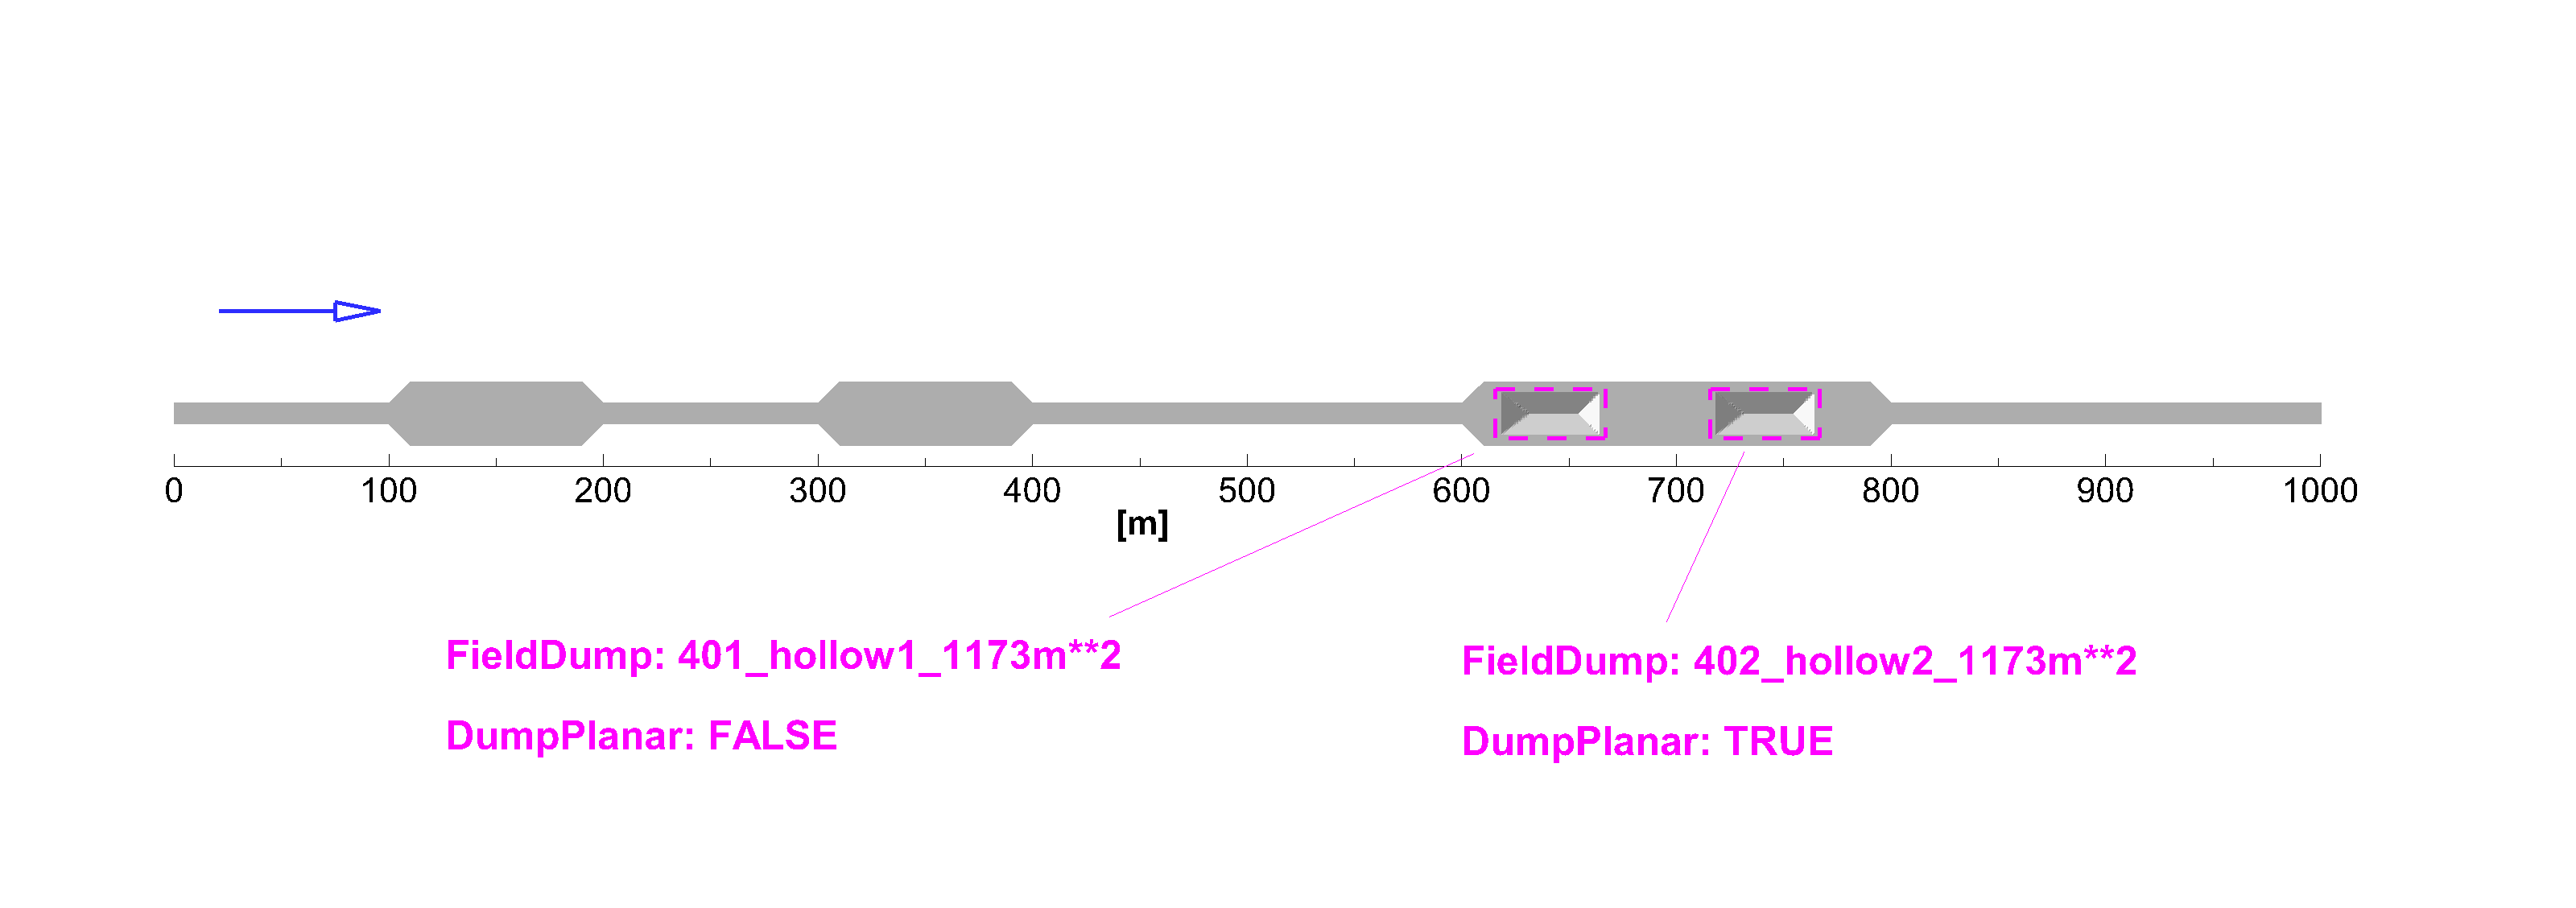
\includegraphics[scale=0.14]{img/result000.png}
 \caption{Geometry of the test flume with three wide sections, the two hollows and the two polygons}\label{E2ini}
\end{figure}


%****************************************************
% - Initial and boundary conditions:
\subsection{Initial and Boundary Conditions}
%
Steady state boundary conditions:\\
\hspace*{3mm} - Discharge at the inlet = 20\,m$^3$/s\\
\hspace*{3mm} - Water depth at outlet = 1\,m\\
\hspace*{3mm} - Sedimentological equilibrium at the inlet (bottom level is constant,\\
\hspace*{5.3mm} bedload transport will be calculated)\\
\\
Initial hydraulic conditions:\\
\hspace*{3mm} - Fully developed flow from a previous simulation is used as initial hydraulic condition.\\
\\
Initial morphological conditions:\\
\hspace*{3mm} - The computation starts with a ground composition which is set in the \\
\hspace*{5.3mm} \textsc{Sisyphe Steering File} and in the Fotran files \texttt{user\_init\_compo.f}\\
\hspace*{5.3mm} and \texttt{user\_noerod.f}.\\
\hspace*{5.3mm} (\textsc{Gaia Steering File} and in the Fotran file \texttt{user\_bed\_init\.f}.)\\


\newpage
%****************************************************
% - Results:H
\section{Results}
%
Figure~\ref{E2result50} shows the evolution after 0s, 70s and 150s. The dumping process finished at 122s.

% Here is an example of how to include the graph generated by validateTELEMAC.py
% They should be in test_case/img
\begin{figure} [H]
\centering
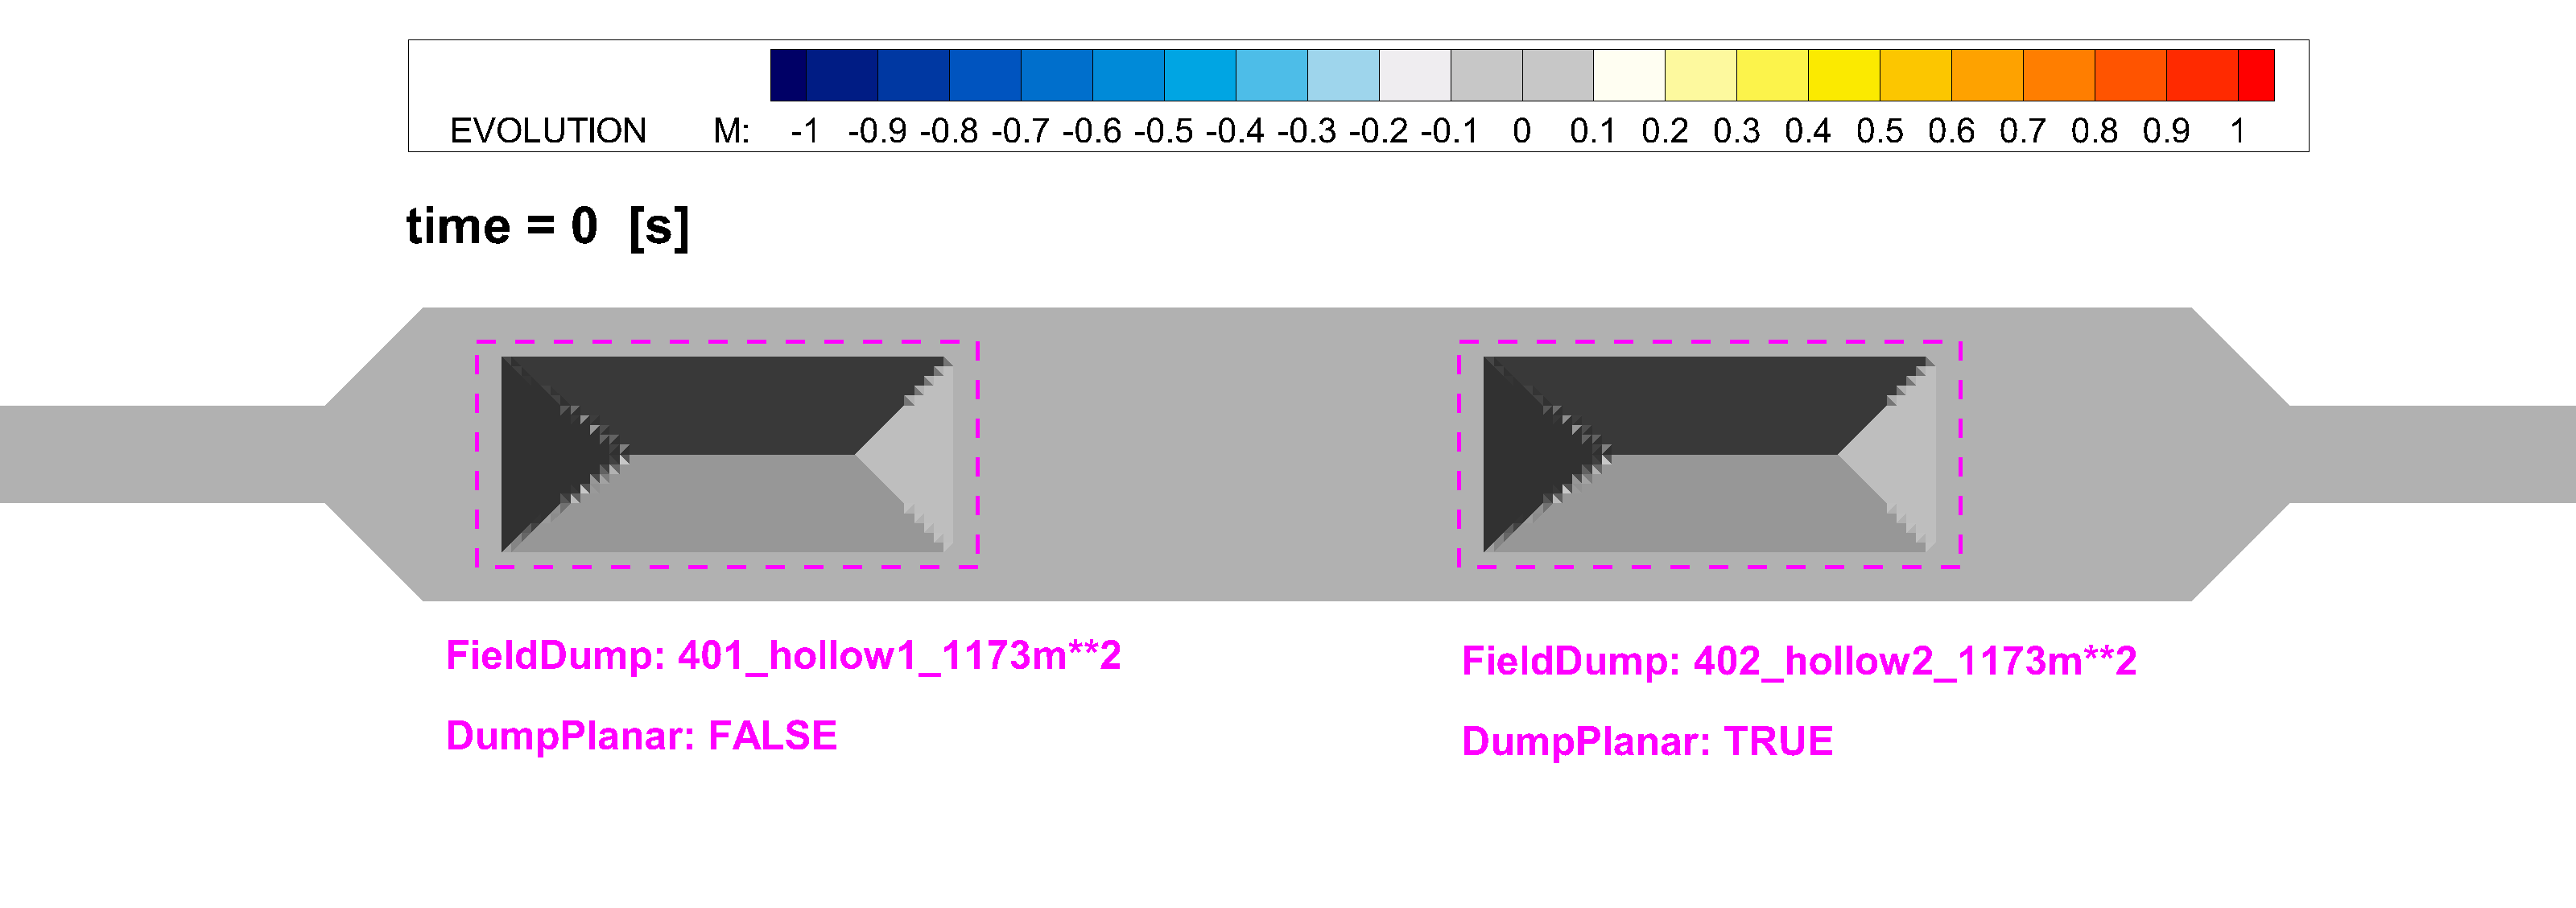
\includegraphics[scale=0.14]{img/result000_zoom.png}
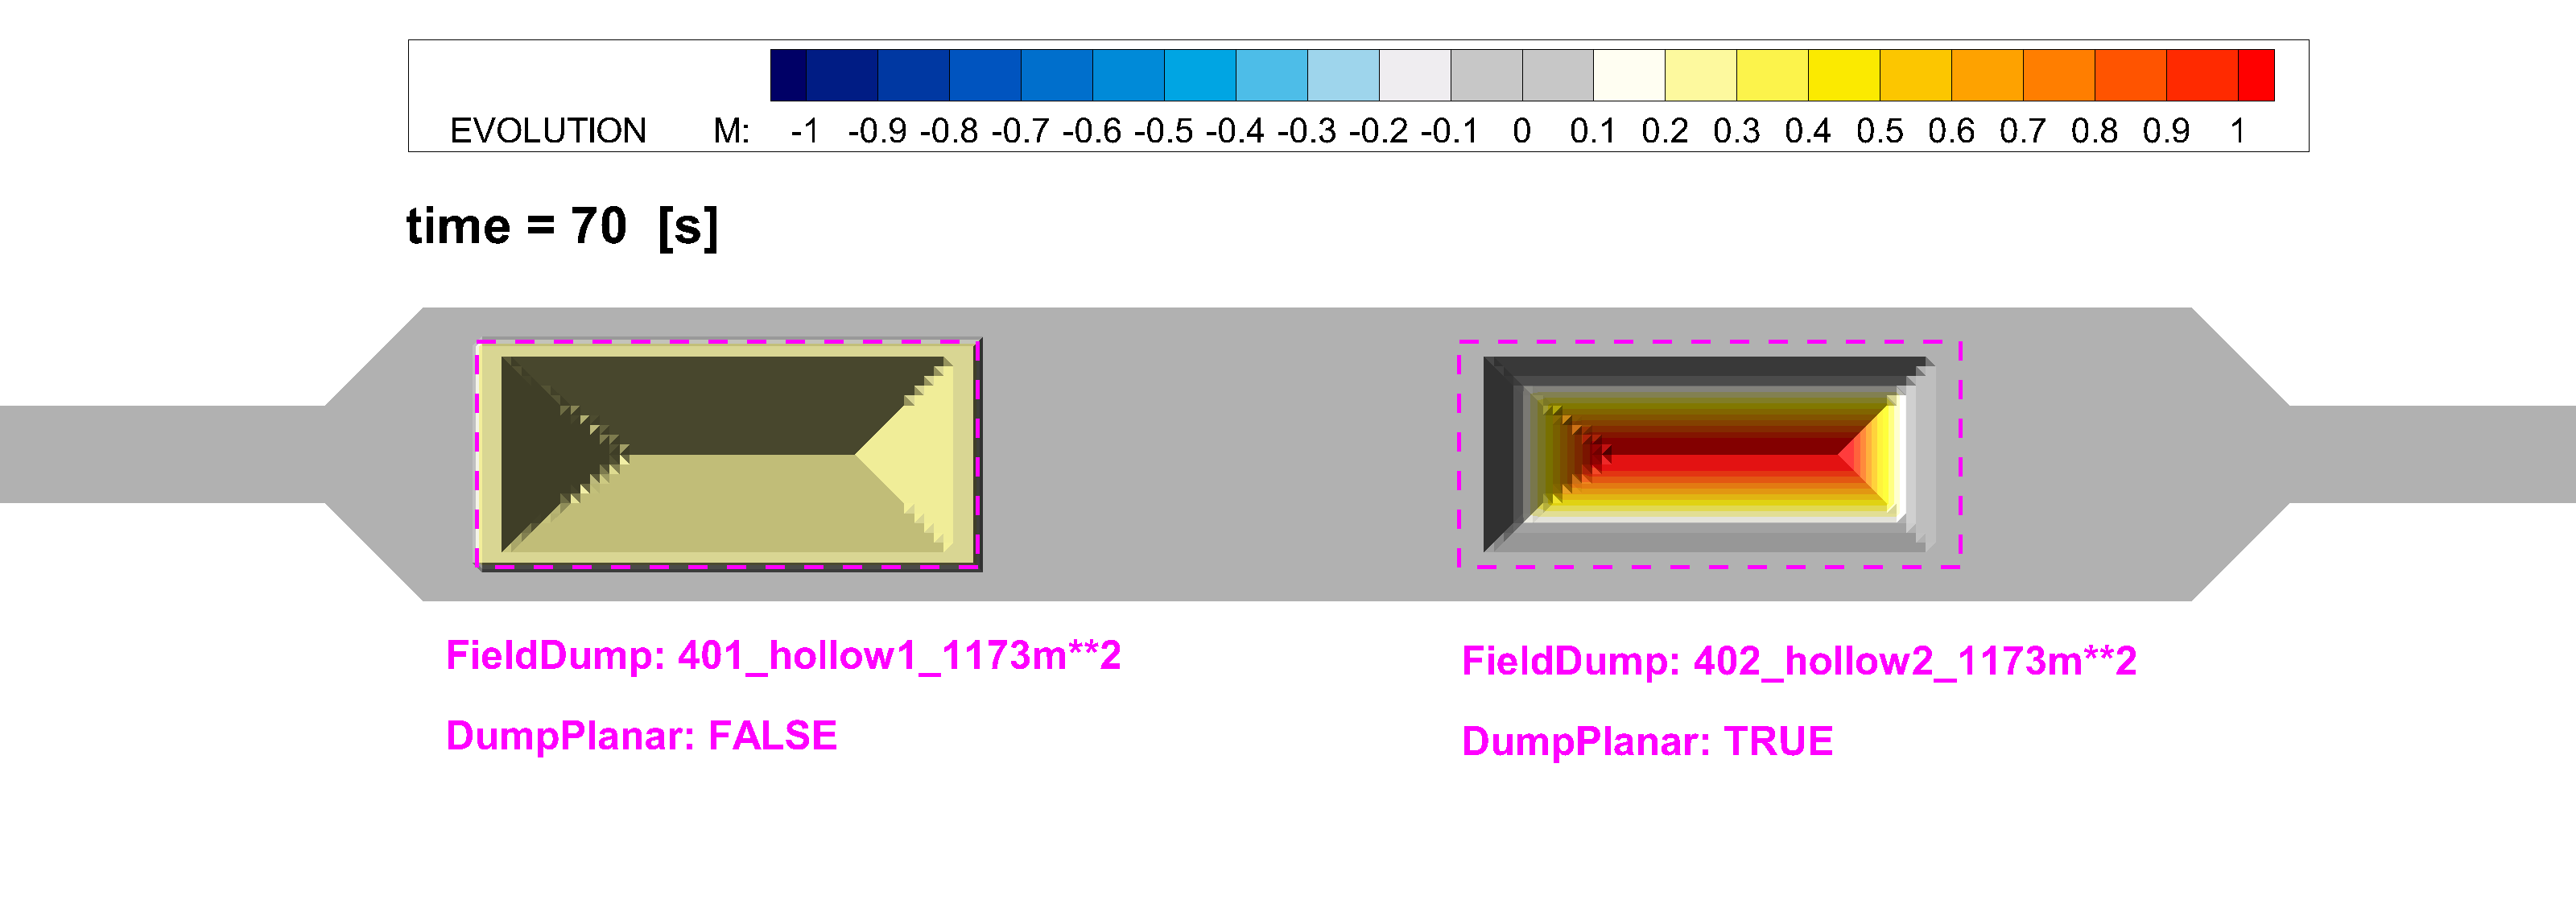
\includegraphics[scale=0.14]{img/result070_zoom.png}
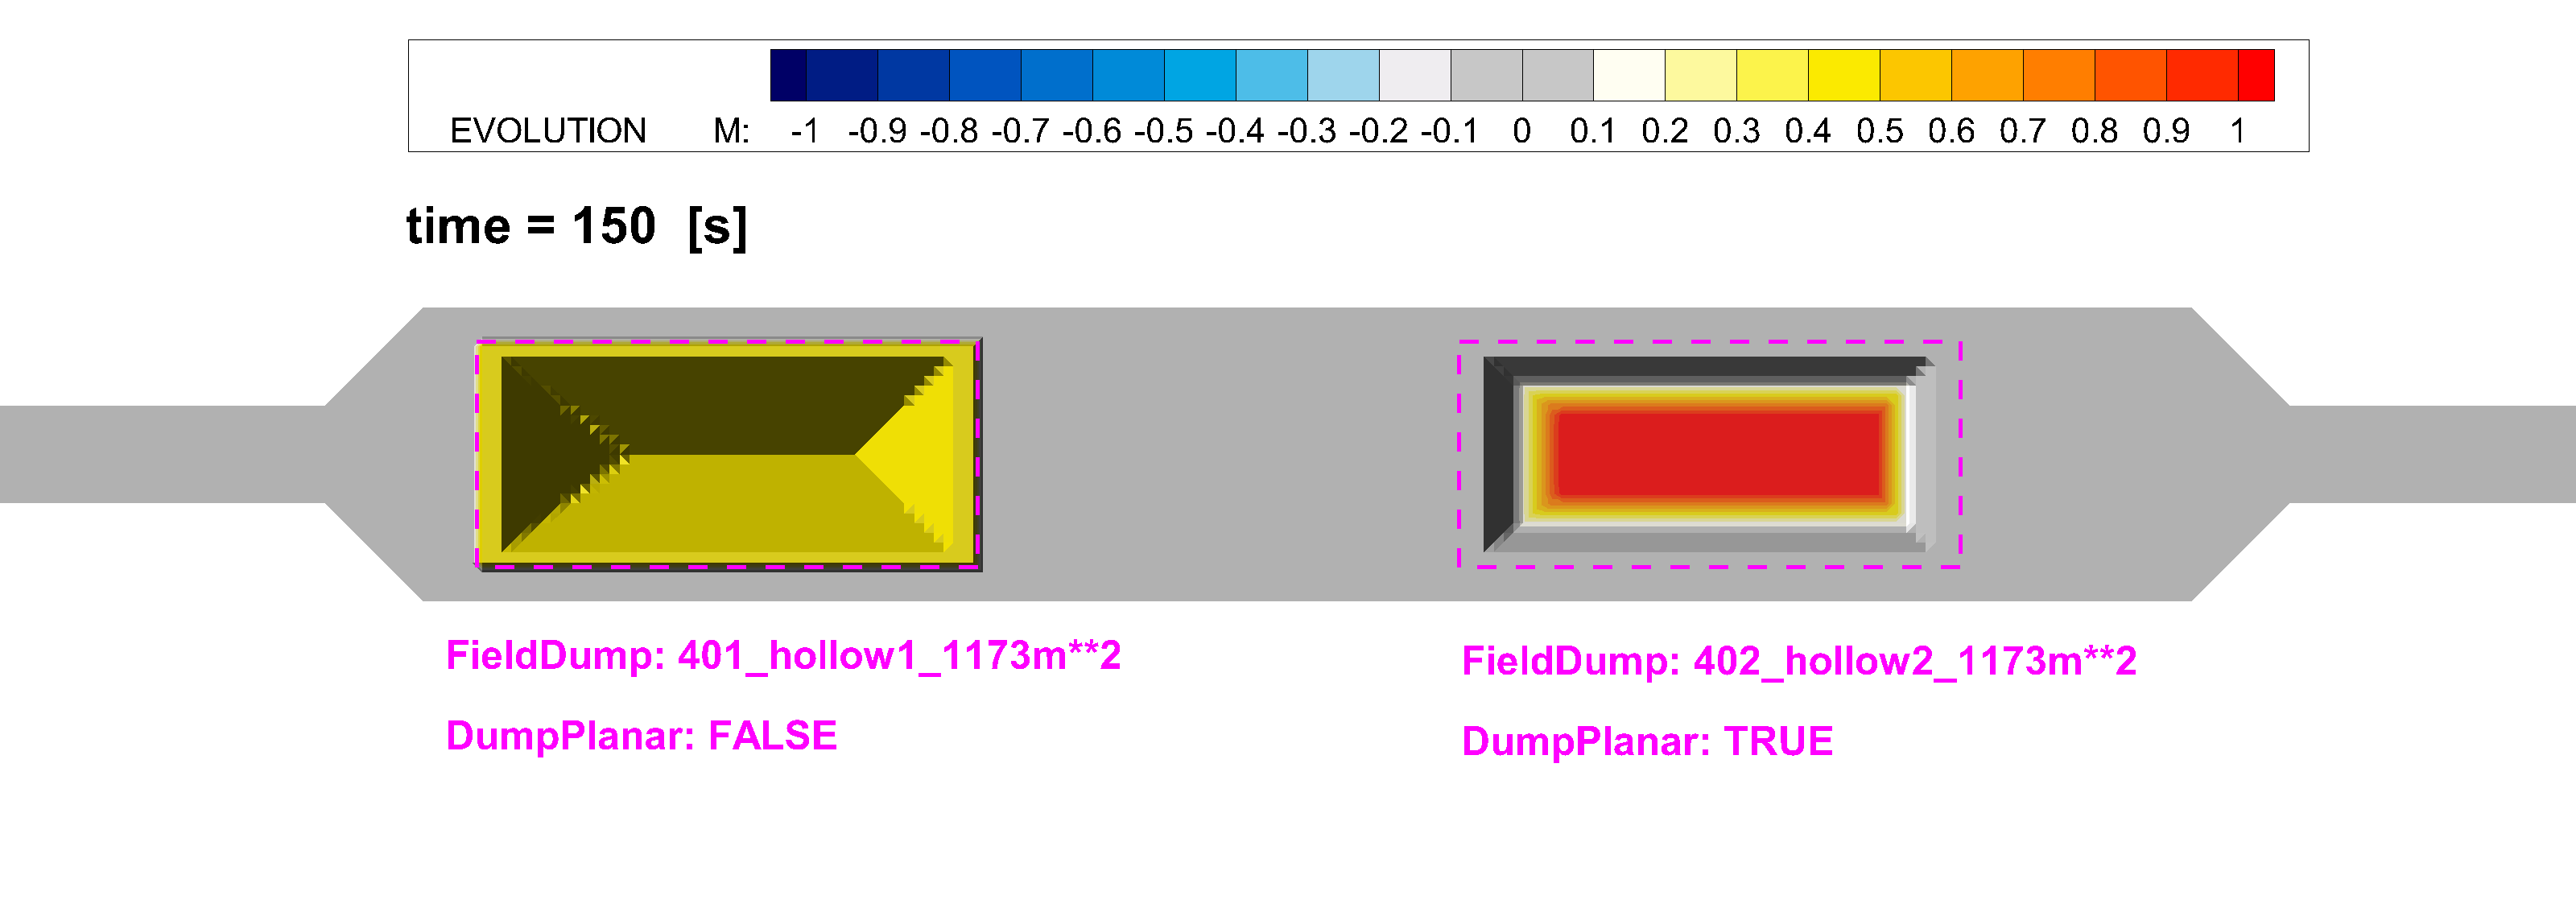
\includegraphics[scale=0.14]{img/result150_zoom.png}
\caption{Simulated evolution after 0\,s, 70\,s and 150\,s.}\label{E2result50}
\end{figure}


\newpage

Figure~\ref{E2result3D} shows the evolution after 0\,s and 150\,s as 3D view.
\begin{figure} [H]
\centering
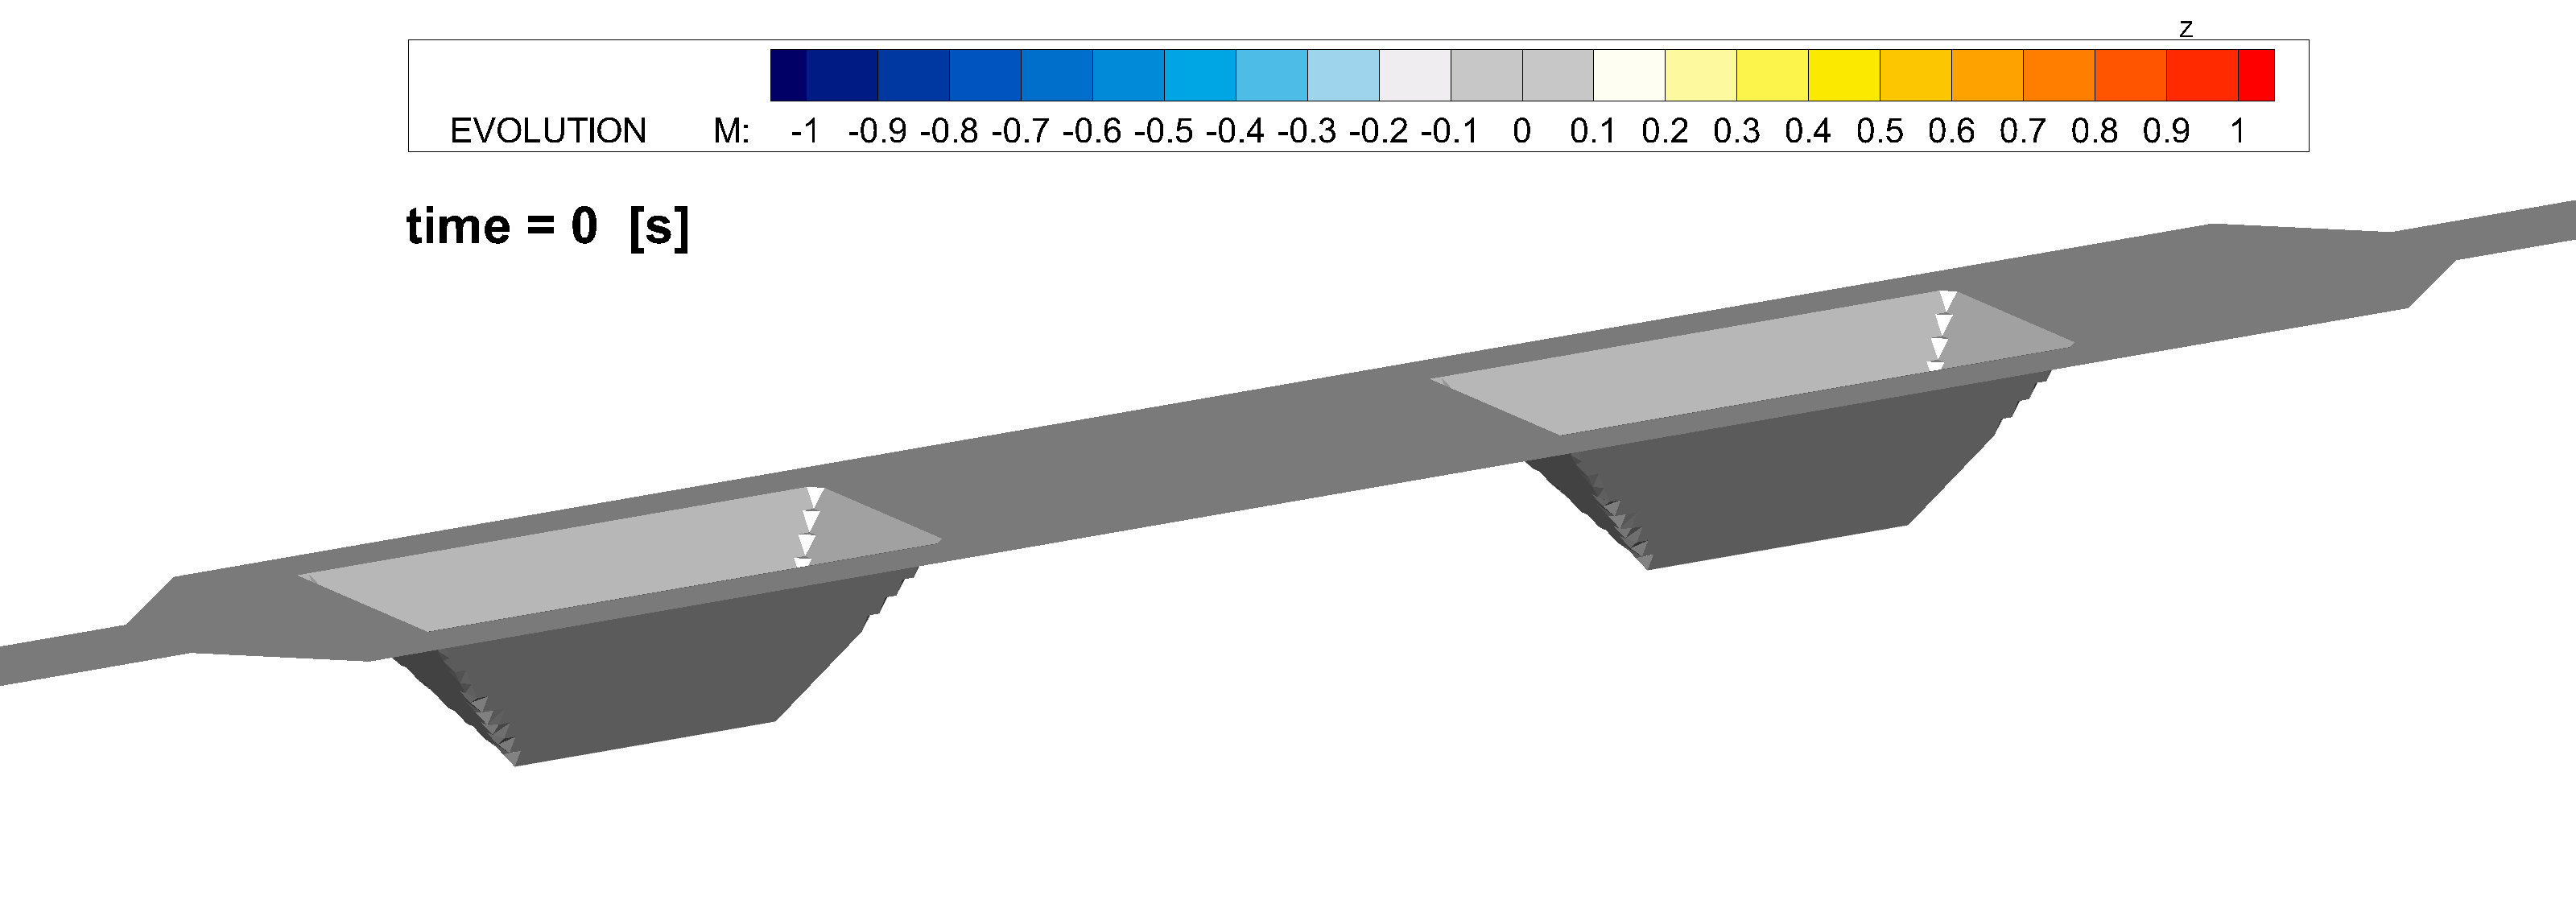
\includegraphics[scale=0.14]{img/result000_zoom3D.png}
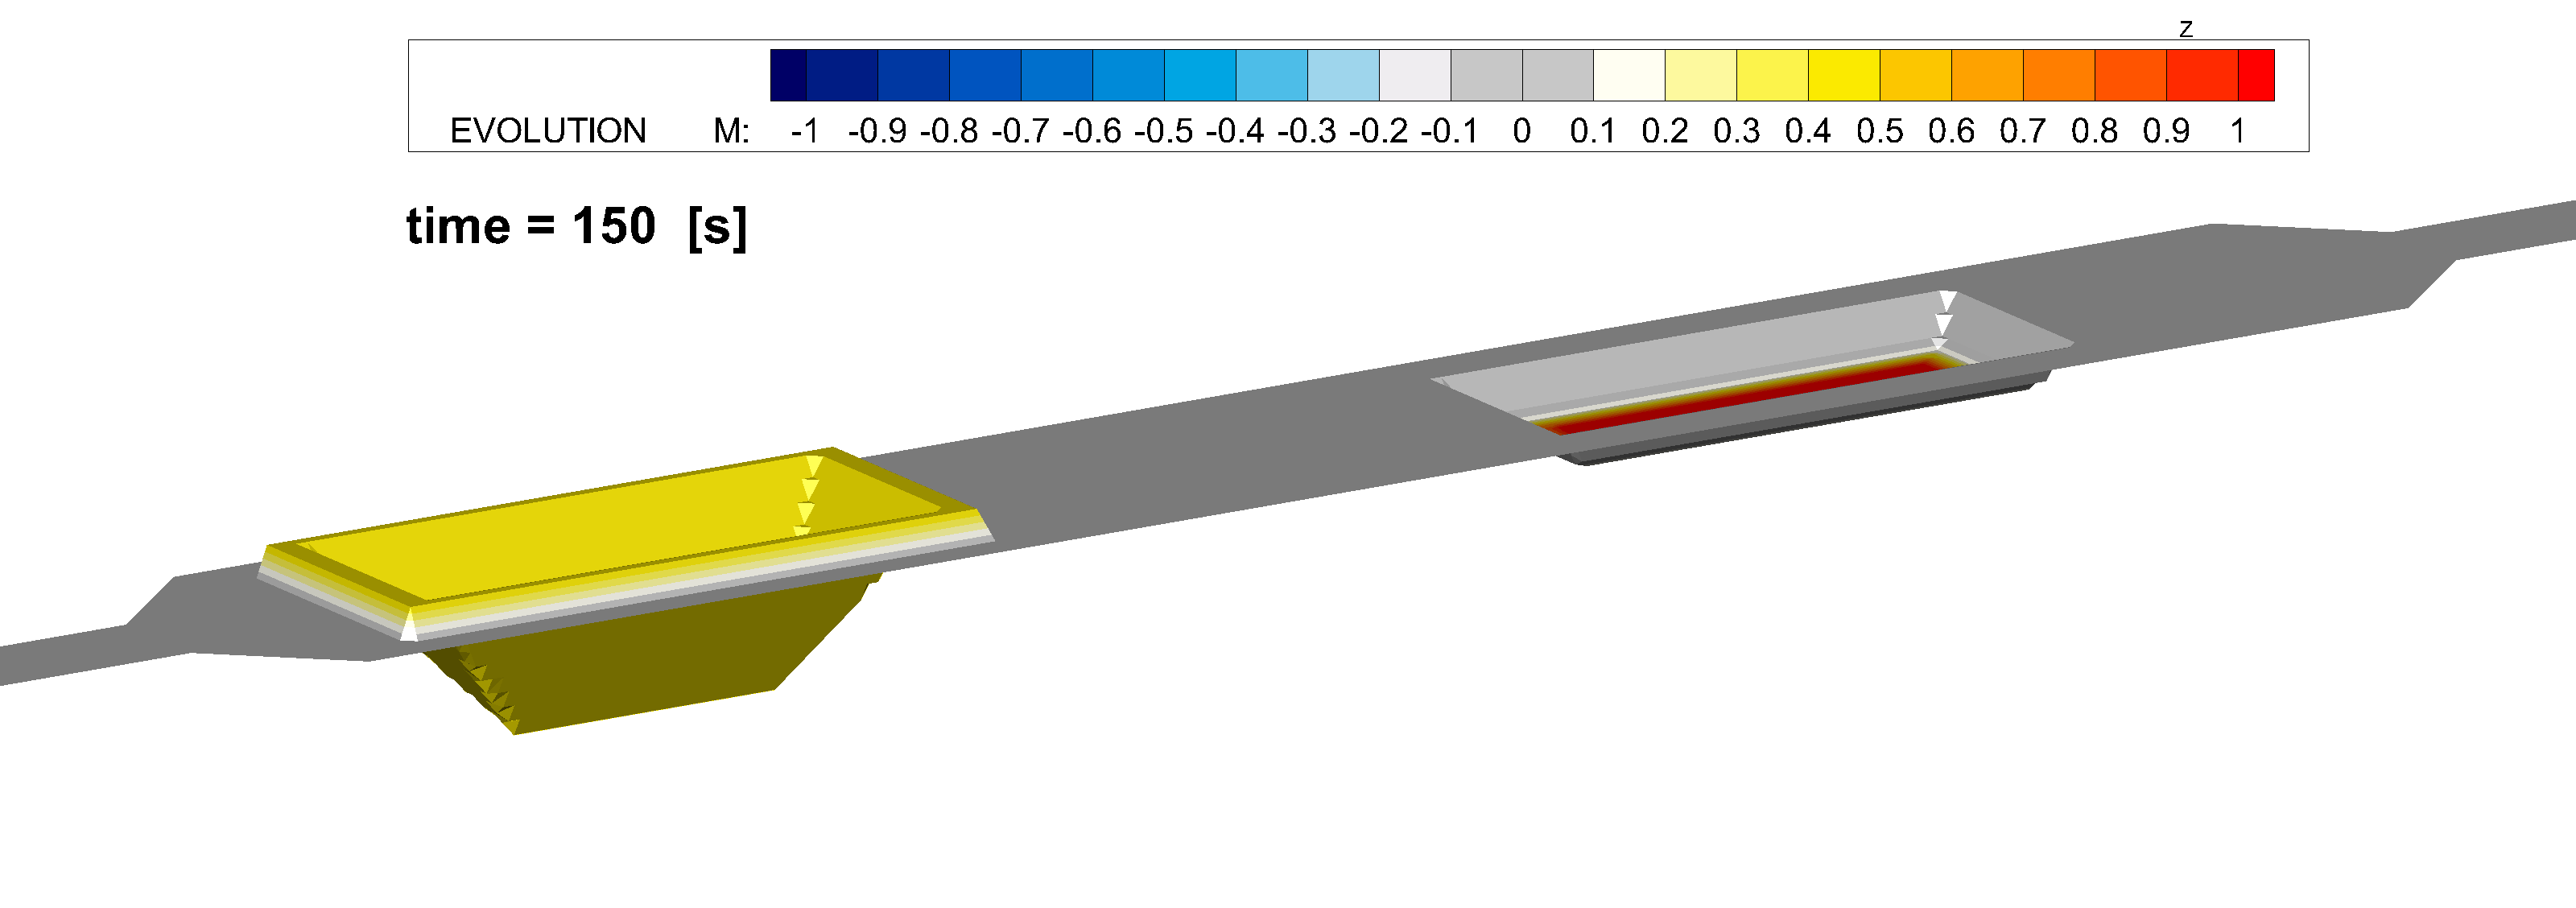
\includegraphics[scale=0.14]{img/result150_zoom3D.png}
\caption{Simulated evolution after 0\,s and 150\,s.}\label{E2result3D}
\end{figure}
